\section{Metodologia}

\subsection{Amostragem}
\begin{frame}
	\frametitle{Dados da amostragem}
	\begin{itemize}
		\item De 11 de novembro de 2006 à 15 de agosto de 2008;
		\item Medidas de 48 horas;
		\item As amostras foram coletadas em filtro de composição de politetrafluoretileno
		(PTFE);
		\item amostradores tipo Harvard (seleção do diâmetro por impactação inercial);
		\item 2898 amostras coletadas de $MP_{10}$ e $MP_{2,5}$ no projeto global e 879 amostras no bairro de Nima;
		\item Onze sítios localizados em quatro bairros diferentes;
		\item Em Nima, dois pontos de amostragem: residencial e avenida;
	\end{itemize}
\end{frame}

\begin{frame}
  \frametitle{Amostragem}
 \begin{center}
  Pontos de amostragem em Nima:
 \end{center}
  \begin{figure}[H]
    \centering
    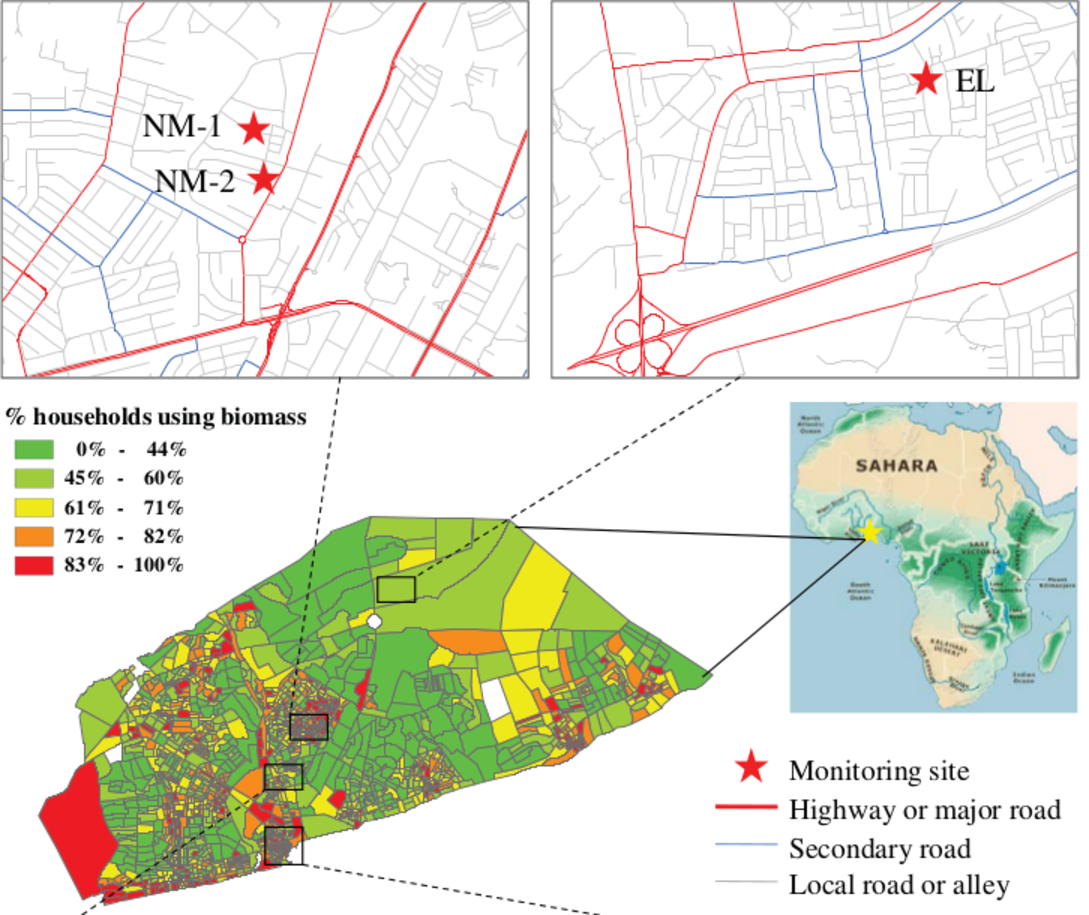
\includegraphics[scale=0.35]{../../inputs/images/zheng/nima_mapa.pdf}
  \end{figure}
\end{frame}

\begin{frame}
  \frametitle{Amostragem}
  \begin{figure}[H]
  \centering	
  \includegraphics[width=0.7\textwidth]{../../outputs/accra_sources.pdf}
  \caption{Levantamento de algumas fontes poluidora de Acra.
           \label{fg:acrasources}}
 \end{figure}
\end{frame}

\begin{frame}
  \frametitle{Censo populacional}
\begin{center}
  Fonte de energia na preparação alimentos em Gana:
\end{center}
  \begin{table}[H]
  	\centering
  	\begin{tabular}{llrlr}
  \hline
  \multicolumn{1}{c}{Tipo da} & \multicolumn{2}{c}{Gana (todo país)} & \multicolumn{2}{c}{Acra}                                                           \\
  \multicolumn{1}{c}{fonte de energia} & 2000 & 2010 &  2000 & 2010  \\ 
 \hline & \multicolumn{4}{c}{\% de uso} \\ 
  \hline
  não cozinha           & 3,5 & 5,60 & 4,8 & 6,90 \\ 
\textcolor{red}{biomassa}              & \textcolor{red}{55,8} & \textcolor{red}{40,20} & \textcolor{red}{8,8} & \textcolor{red}{3,50} \\ 
\textcolor{blue}{gás}& \textcolor{blue}{6,2} & \textcolor{blue}{18,20} & \textcolor{blue}{21,8} & \textcolor{blue}{41,40} \\ 
  eletricidade          & 1,1 & 0,50 & 2,2 & 0,90 \\ 
  querosene             & 2 & 0,50 & 4,3 & 1,10 \\ 
 \textcolor{red}{carvão} & \textcolor{red}{30} & \textcolor{red}{33,70} & \textcolor{red}{57,3} & \textcolor{red}{45,40} \\ 
  resíduo de plantação  & * & 0,80 & * & 0,10 \\ 
  pó de serra           & * & 0,10 & * & 0,30 \\ 
  esterco               & * & 0,00 & * & 0,10 \\ 
  outros                & 1,1 & 0,10 & 0,8 & 0,30 \\ 
  \hline
\end{tabular}


  \end{table}
\end{frame}

\subsection{Fluorescência de raios X}
\begin{frame}
  \frametitle{Fluorescência de raios X}
  Ilustração clássica do fenômeno de fluorescência de raios X no átomo.
  \begin{figure}[H]
    \centering
    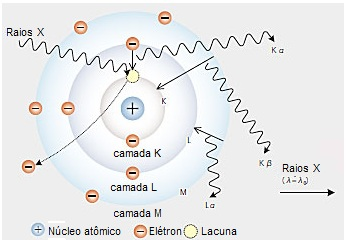
\includegraphics[width=0.4\textwidth]{../../inputs/images/shimadzu_atomo.jpg}
    \hspace{1cm}
    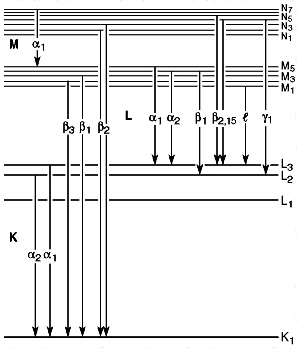
\includegraphics[width=0.4\textwidth]{../../inputs/images/Siegbahn.jpg}
  \end{figure}
\end{frame}

\begin{frame}
	\frametitle{Shimadzu EDX 720HS}
	\begin{itemize}
		\item Shimadzu EDX 720HS (instalada no Lapat);
		\item Tubo de ródio (Rh) submetido a ddp de 50 kV;
		\item Detector de Si(Li) (1 e 20 keV) e multicanal de 2048 canais;
		\item Filtro de Al para remoção da linha L do feixe do tubo de ródio;
		\item Criação de suporte fixação dos filtros. 
	%	\item Tempo vivo de $\pm$ 960 minutos, ajustando-se a corrente para manter o tempo morto em 20\%;
	\end{itemize}
	\begin{figure}[H]
		\centering
		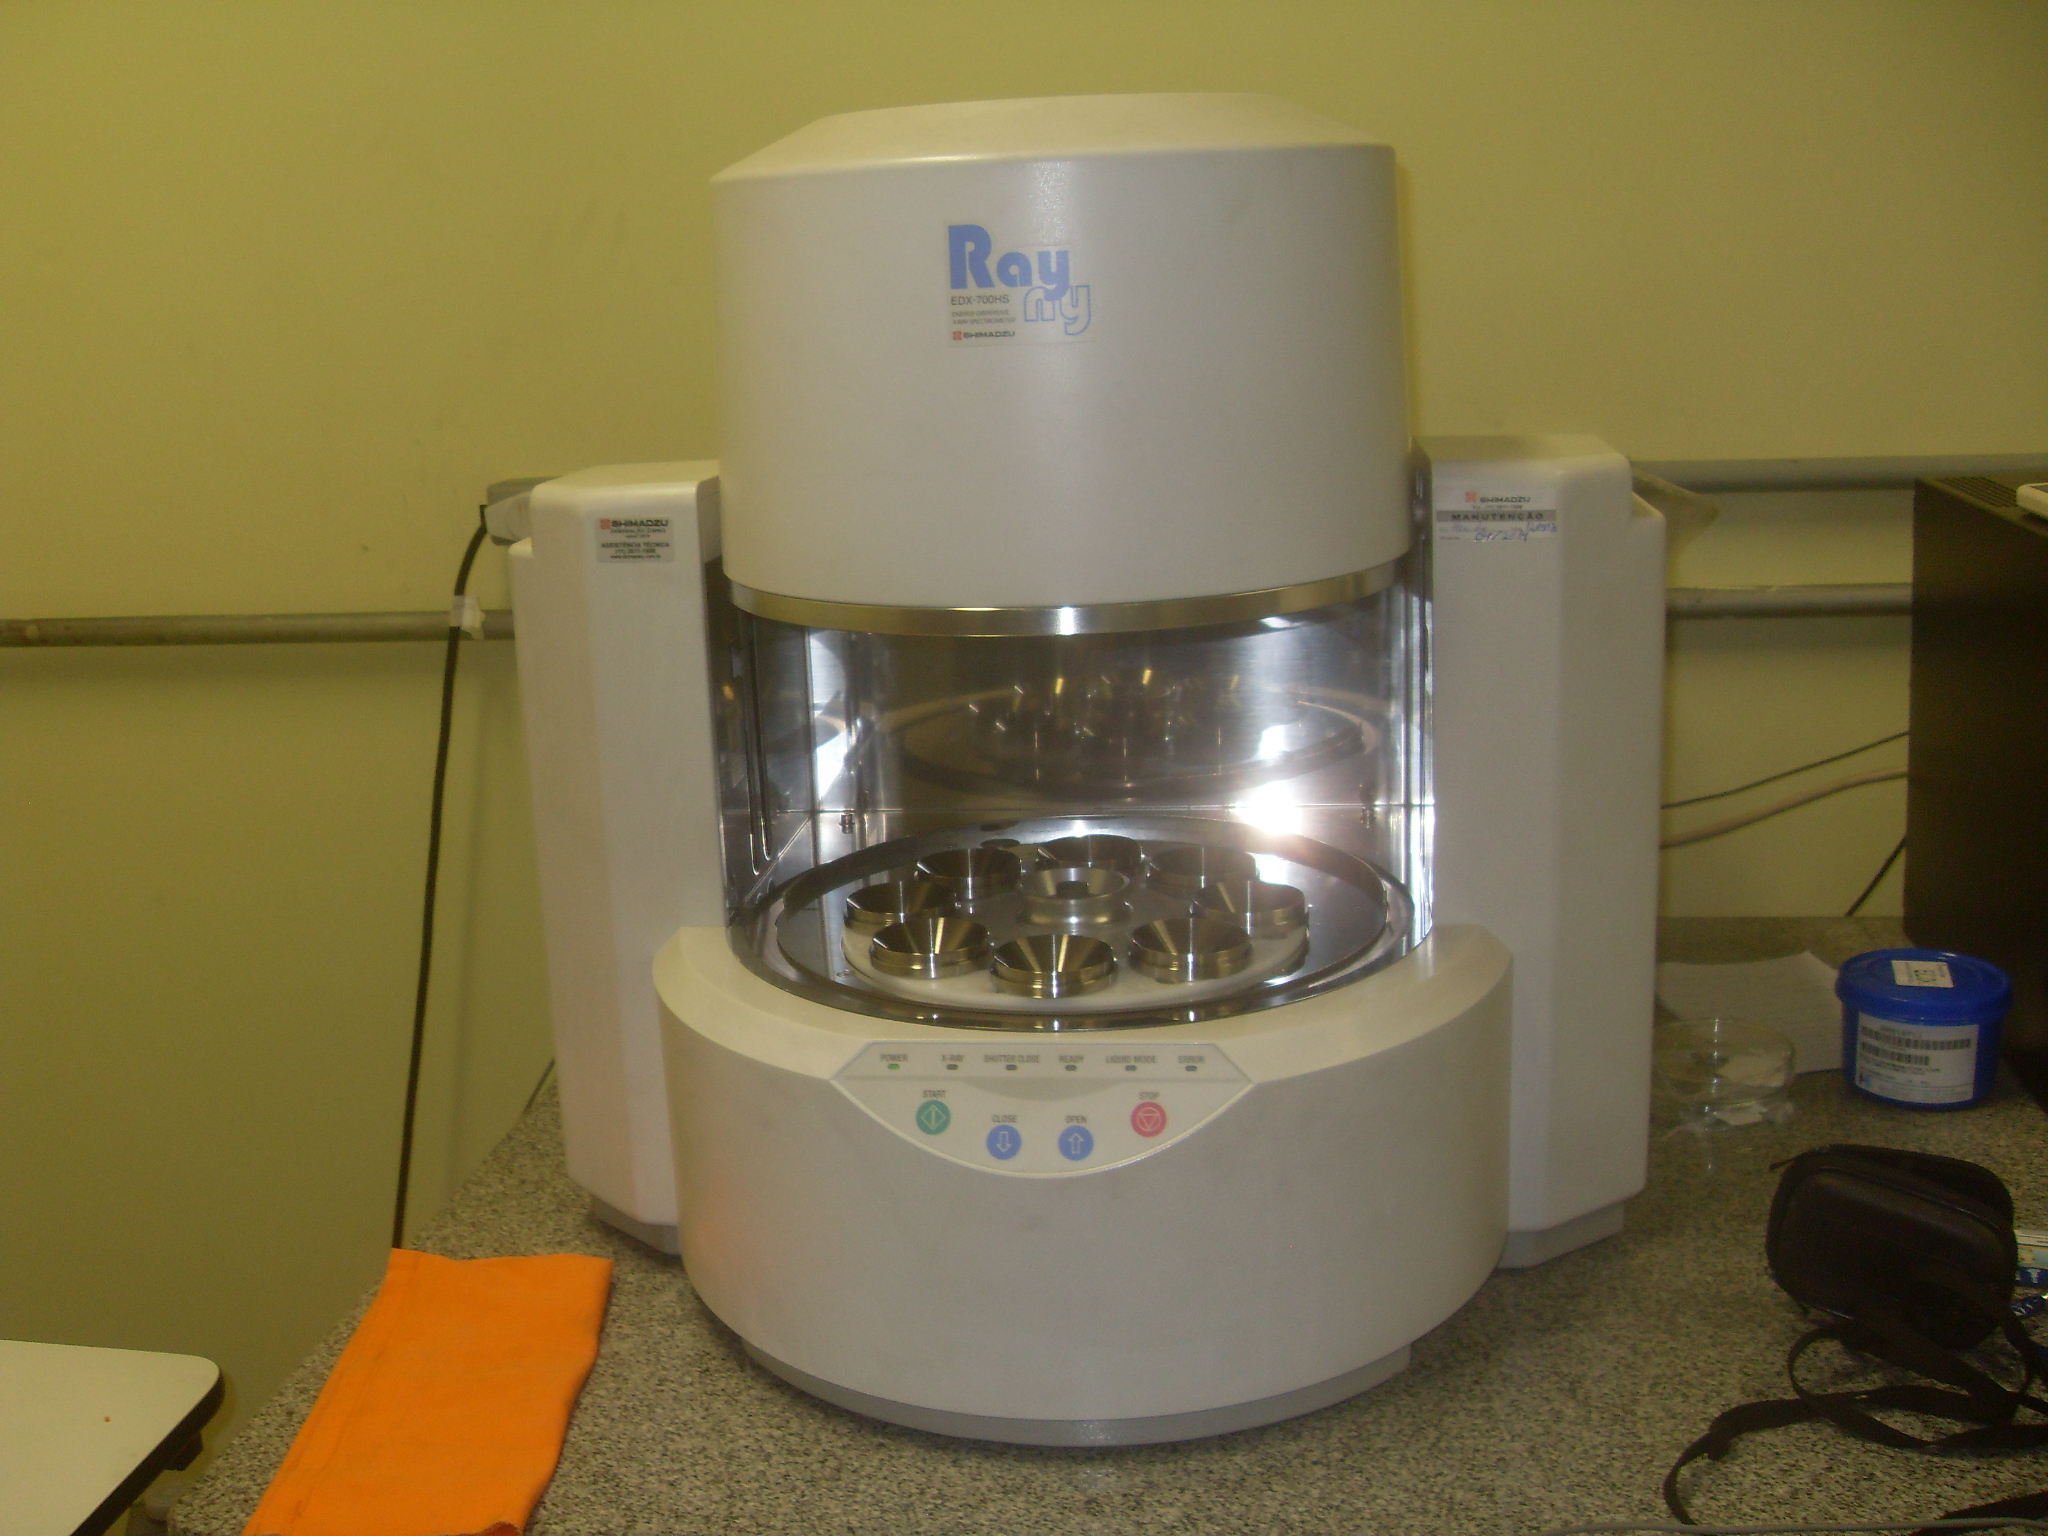
\includegraphics[width=0.4\linewidth]{../../inputs/images/xrf-ed-IAG-USP.jpg}
		\hspace{0.4cm}
		  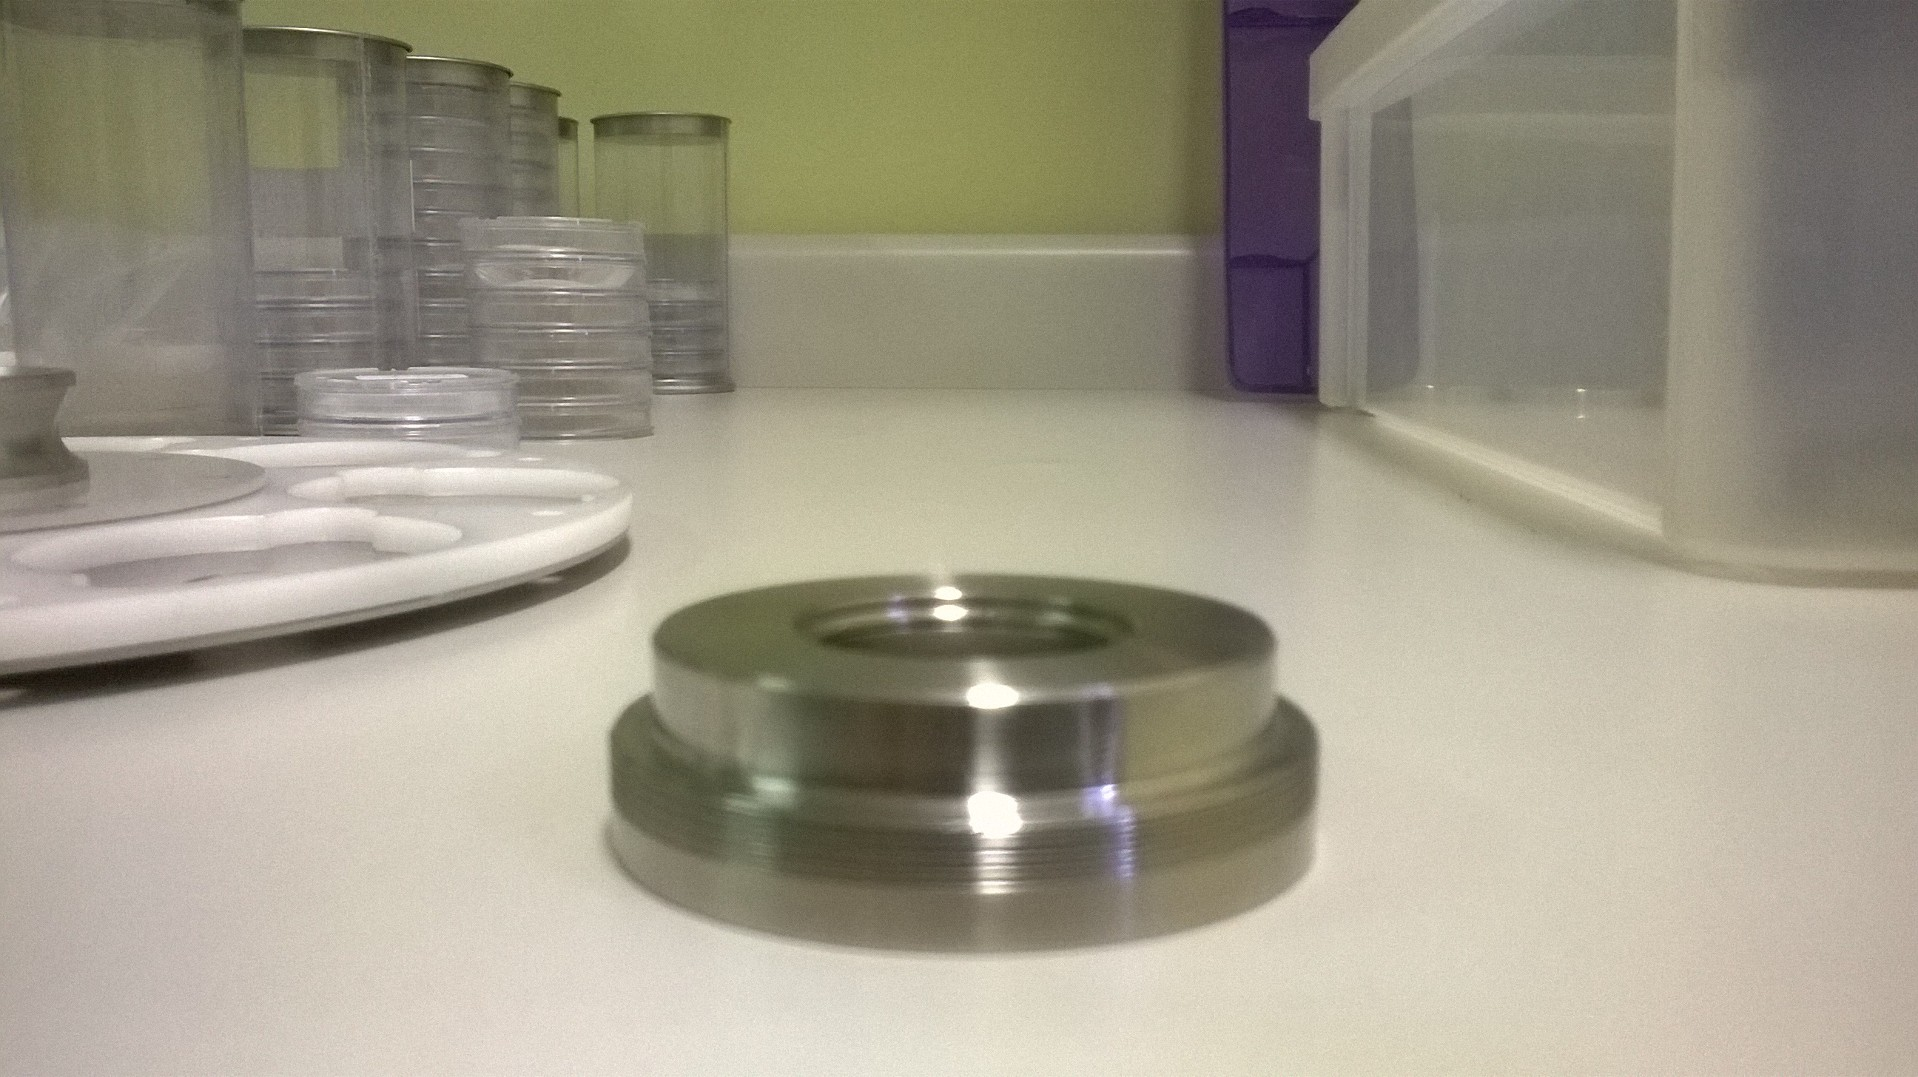
\includegraphics[width=0.4\linewidth]{../../inputs/images/suporte8.jpg}
	\end{figure}
\end{frame}

\begin{frame}
	\frametitle{Espectro no WinQxas}
\begin{figure}[H]
	\centering
	\begin{subfigure}[b]{0.7\textwidth}
		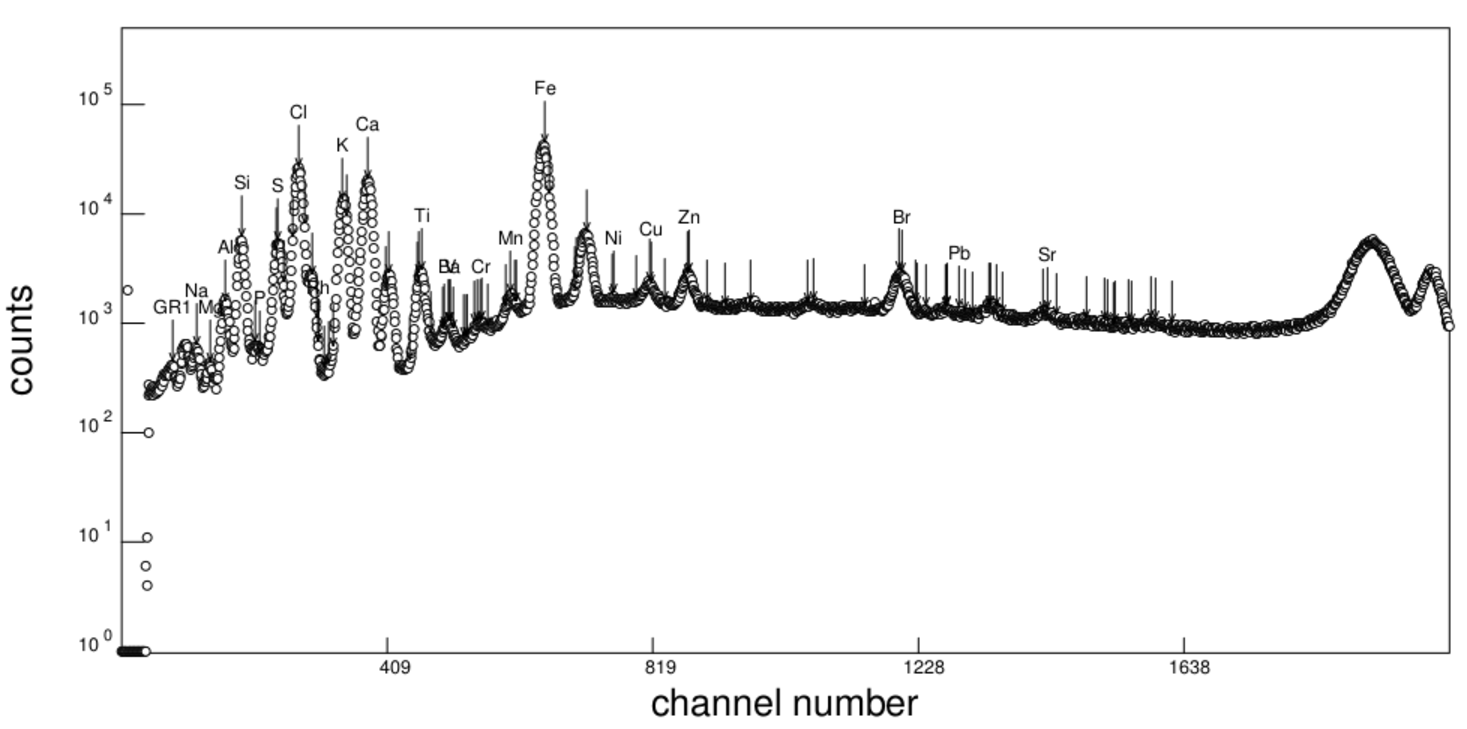
\includegraphics[width=\textwidth]{../../inputs/images/winqxas/GHA41editado.pdf}
	\end{subfigure}
	\begin{subfigure}[b]{0.7\textwidth}
		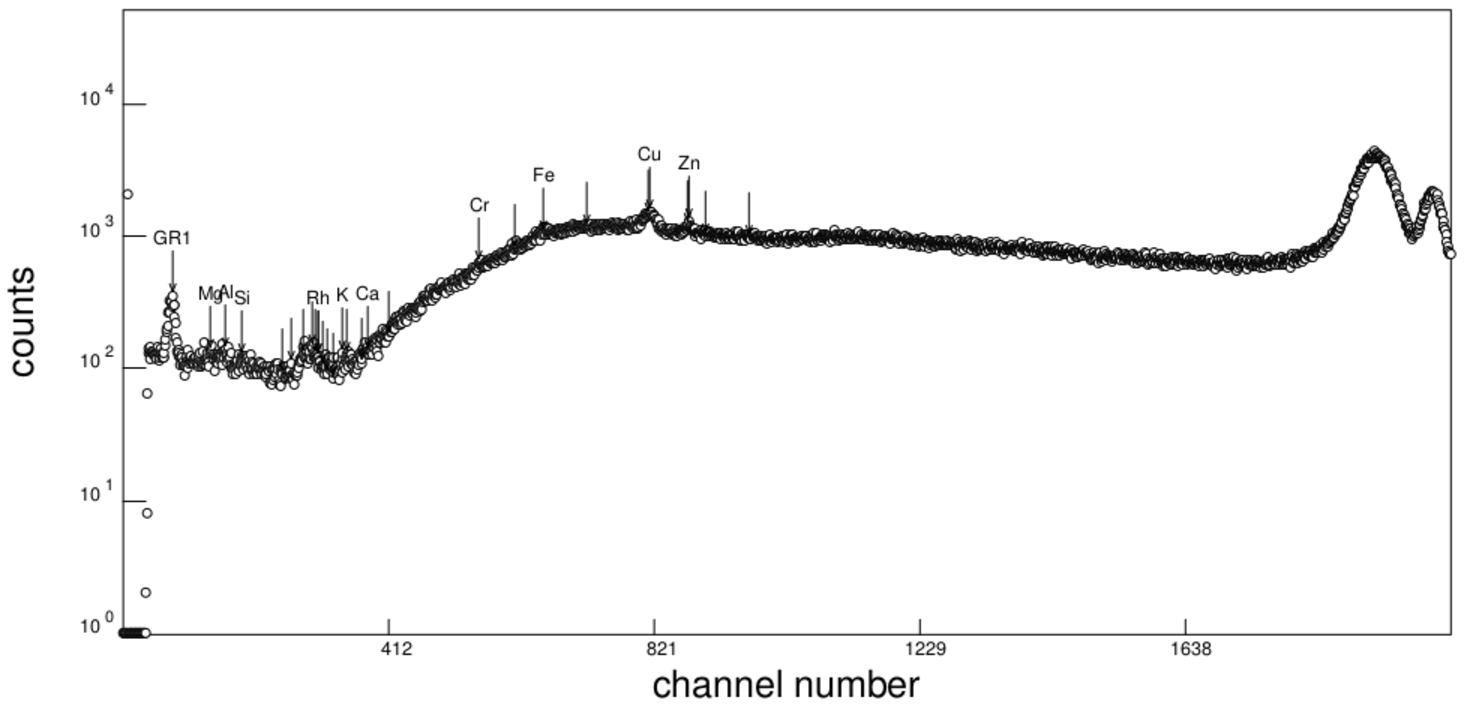
\includegraphics[width=\textwidth]{../../inputs/images/winqxas/GPE770editado.pdf}
	\end{subfigure}
\end{figure}
\end{frame}

\begin{frame}
  \frametitle{Fluorescência de raios X}
  \begin{equation*}
    \label{eq:contagem}
    N(Z) = R(Z) \cdot I \cdot \Delta t  \cdot \frac{m(Z)}{A}
  \end{equation*}
  Onde,  
  \begin{itemize}
    \item N(Z) = Contagem de fótons na amostra para o elemento químico Z;
    \item I = Corrente (ampère) na amostra;
    \item $\Delta t$ = Tempo vivo (segundos) que a amostra foi irradiada;
    \item m(Z) = Massa na amostra para o elemento químico Z;
    \item A = Área amostrada do filtro;
    \item R = Fator de Resposta.
  \end{itemize}
\end{frame}

\begin{frame}
  \frametitle{Fator de Resposta a partir de alvos padrões}
  \begin{footnotesize}
  \begin{equation*}
    R(Z) = \frac{N(Z)}{d(Z) \cdot I \cdot \Delta t}
  \end{equation*}
    
  \begin{equation*}
  \sigma_{R(Z)}^2 = {R(Z)}^2 \cdot \left[ \left(\frac{\sigma_{N(Z)}}{N(Z)}\right)^2 + 
  \left(\frac{\sigma_{d(Z)}}{d(Z)}\right)^2 
  \right]
  \end{equation*}
\end{footnotesize}  
  \begin{figure}[H]
  	\begin{subfigure}[b]{0.4\textwidth}
  		\includegraphics[width=\textwidth]{../../outputs/plot_R_maio2010K.pdf}
  		\caption{linha K}
  	\end{subfigure}%
  	\begin{subfigure}[b]{0.4\textwidth}
  		\includegraphics[width=\textwidth]{../../outputs/plot_R_maio2010L.pdf}
  		\caption{linha L}
  	\end{subfigure}
  \end{figure}
\end{frame}

\begin{frame}
  \frametitle{Massa Elementar}
\begin{equation*}
  \label{eq:xrfedmassa}
  m(Z) = \frac{N(Z) \cdot A}{ R(Z) \cdot I \cdot \Delta t}
\end{equation*}

\begin{equation*}
  \label{eq:erro_massa}
  \sigma_{m(Z)}^2 = {m(Z)}^2 \left[ \left(\frac{\sigma_{N(Z)}}{N(Z)}\right)^2 + 
                                  \left(\frac{\sigma_A}{A}\right)^2 + 
                                  \left(\frac{\sigma_{R(Z)}}{R(Z)}\right)^2 
                             \right]
\end{equation*}
\end{frame}

\begin{frame}
  \frametitle{Mínimos Quadrados Matricial} 
\begin{equation*}
  \label{eq:polinomio}
  \begin{split}
    y_1 = a + b x_1 + c{x_1}^2 + d{x_1}^3 + ...\\
    y_2 = a + b x_2 + c{x_2}^2 + d{x_2}^3 + ... \\
    ...
  \end{split}
\end{equation*}

\begin{equation*}
  \label{eq:polinomioMatriz}
  [Y] = [A] \cdot [X]
\end{equation*}

Os coeficientes ajustados [Ã] são dados por:
\begin{equation*}
  [\tilde{A}] = [V_{\tilde{A}}] \cdot ([X]^T \cdot {[V_Y]}^{-1} \cdot [Y])
\end{equation*}

Sendo $[V_{\tilde{A}}]$ a matriz de covariância dos coeficientes, dada por:
\begin{equation*}
  [V_{\tilde{A}}] = ([X]^T [V_Y]^{-1} [X])^{-1}
\end{equation*}
A incerteza é dada pela diagonal da matriz de covariância de $[\tilde{Y}]$:
\begin{equation*}
\label{eq:matrizcovarianciaY}
[V_{\tilde{Y}}] = [X] \cdot [V_{\tilde{A}}]^{-1} \cdot [X]^{-1}
\end{equation*}
\end{frame}

\subsection{Black Carbon}
\begin{frame}
  \frametitle{Refletância}
  \begin{equation*}
  \label{eq:dIdx}
  \frac{dI}{dx} = -\alpha \cdot I
  \end{equation*}
 
  \begin{equation*}
  \label{m/a_2}
  \frac{m}{A} = K \cdot (2-logI) 
  \end{equation*}
  
% Onde, $K = [2 \cdot ({\alpha}/{\rho}) \cdot log(e)]^{-1}$ e $I_0$ = 100\%.
 
\begin{center}
	 Refletômetro da \textit{Diffusion System} modelo ELL43D:
\end{center}
  \begin{figure}[H]
  	\centering
  	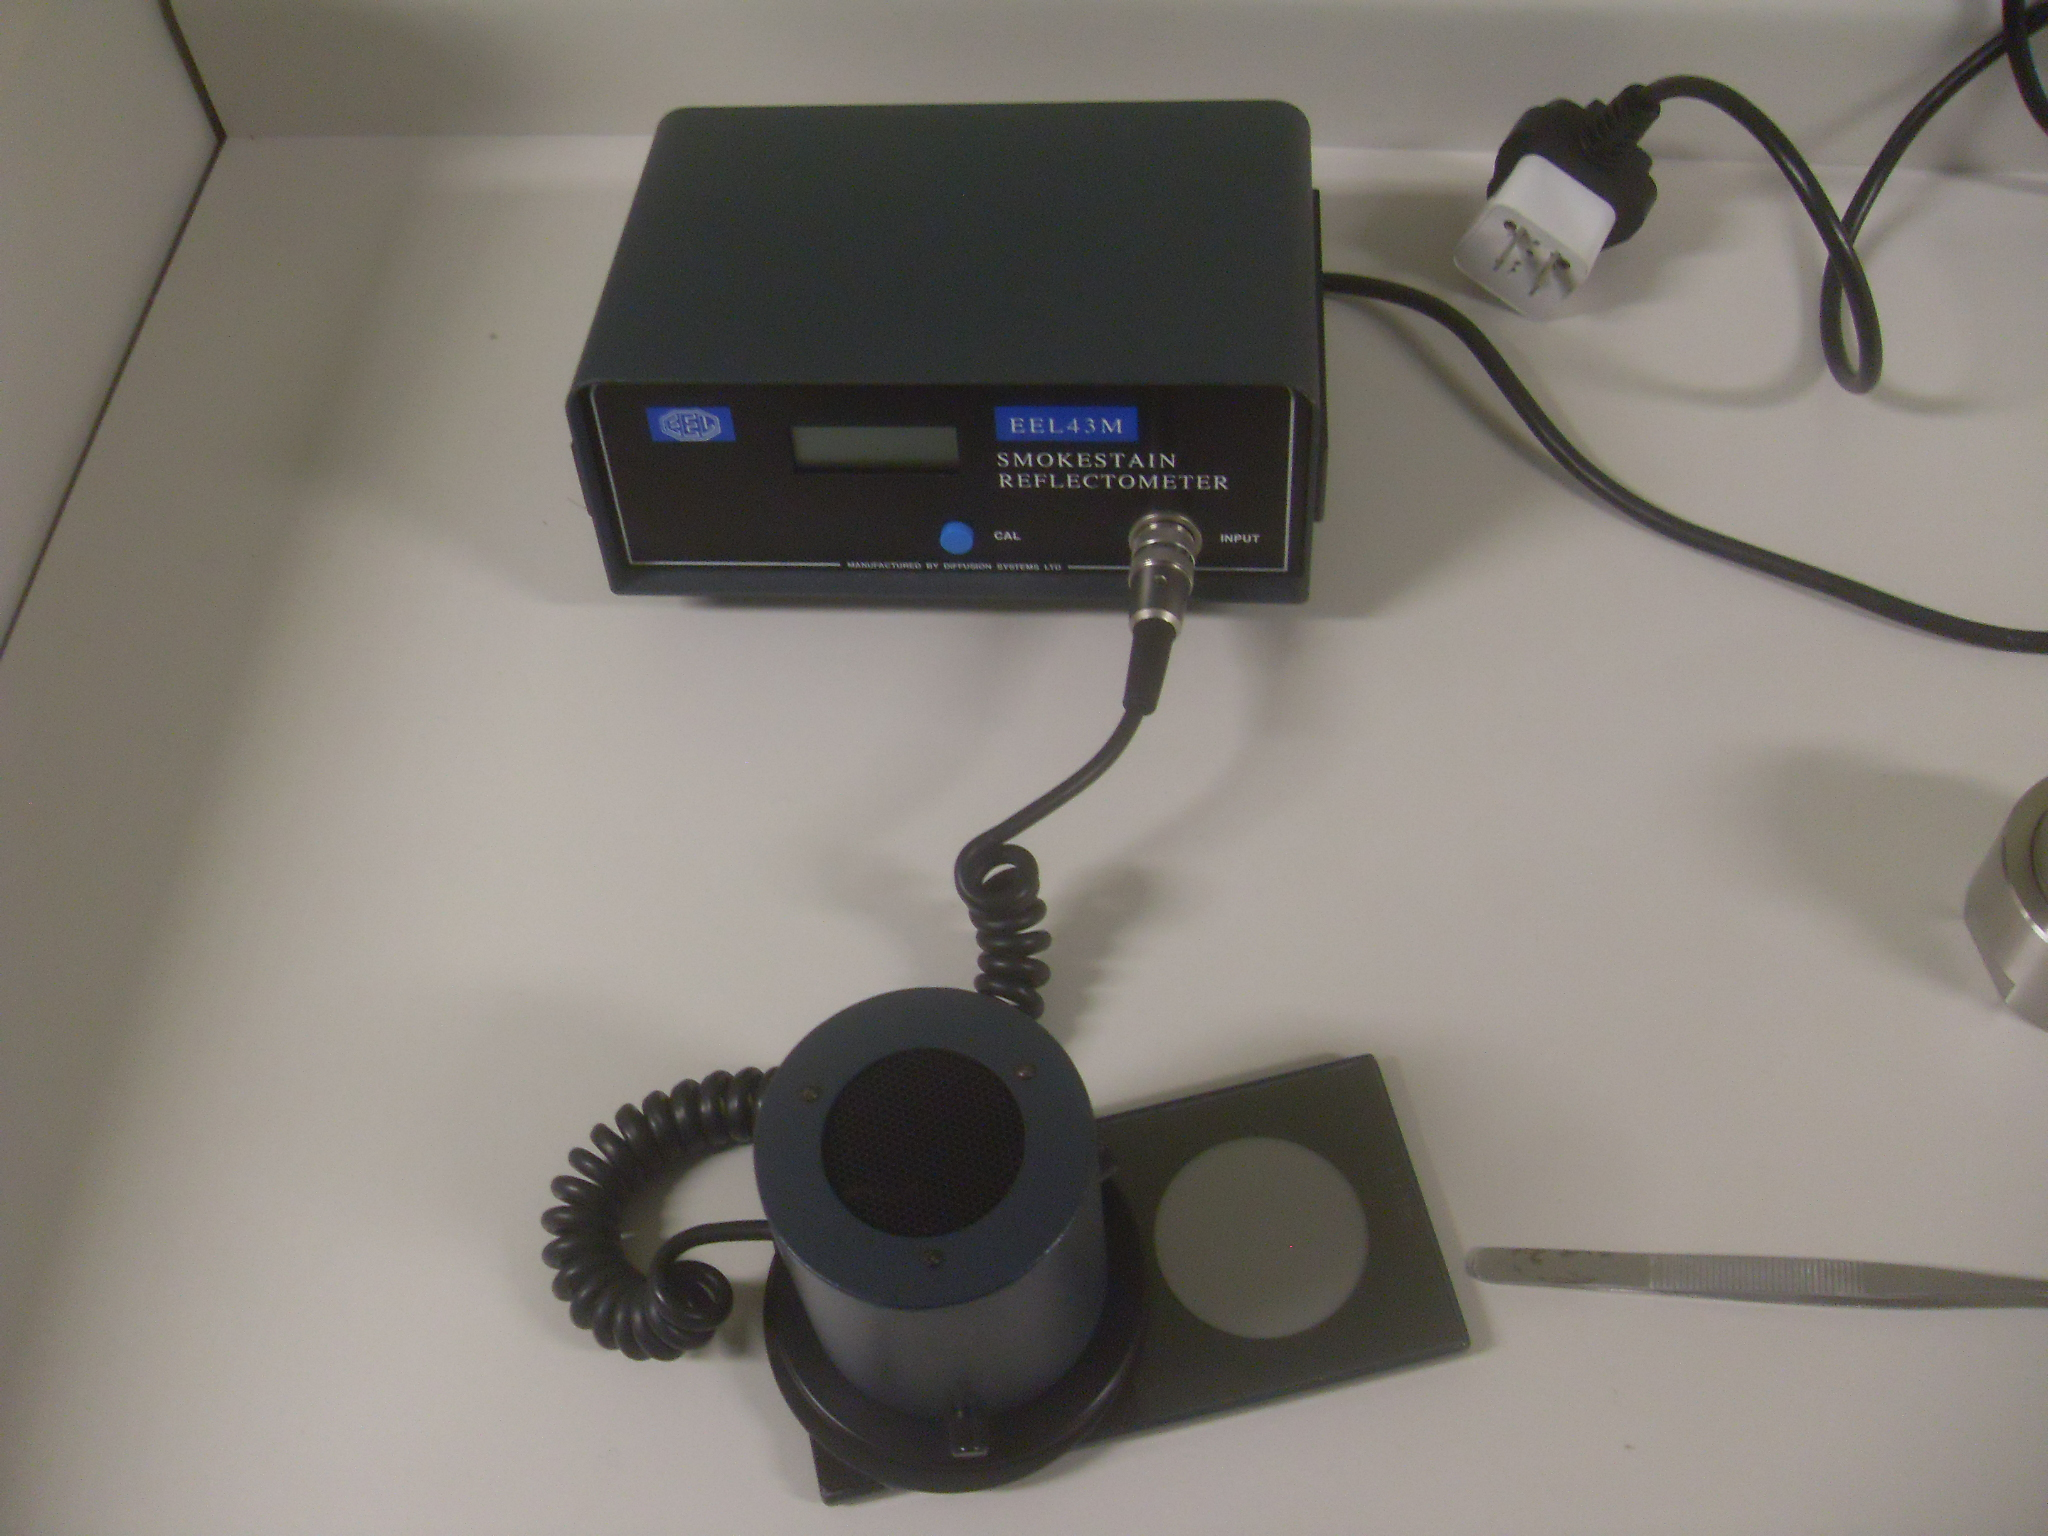
\includegraphics[width=0.38\linewidth]{../../inputs/images/refletometro.jpg}
  \end{figure}
\end{frame}

\subsection{Modelo receptor}
\begin{frame}
  \frametitle{Modelo receptor}
  \textbf{Modelo Receptor} é uma abordagem matemática para quantificar o efeito das fontes 
  nas amostras. Determinar as fontes a partir do receptor. \\
  \textbf{Análise Multivariada} reduz as dimensões (variáveis) de um conjunto de dados 
   analítico complexo que poderão ser interpretados como tipo de fontes. 
   \begin{center}
   	\textbf{Conservação da massa}
   \end{center}
     \begin{equation*}
     x_{ij} = \sum_{p=1}^{P} g_{ip}f_{pj} + \epsilon_{ij}
     \end{equation*} 
     \begin{footnotesize}
    
     \begin{itemize}
     	\item $x_{ij}$ = concentração na amostra i da espécie j;
     	\item $f_{pj}$ = fração da espécie j emitida na fonte/fator p 
     	(perfil da fonte, assinatura da fonte ou \textit{Factor Loadings}); 
     	\item $g_{ip}$ = contribuição da fonte/fator p para amostra i (\textit{Factor Score});
     	\item $\epsilon_{ij}$ = Resíduo, depende do modelo empregado.
     \end{itemize}
         \end{footnotesize}
\end{frame}

\begin{frame}
  \frametitle{Análise de Fatores}
\begin{equation*}
\label{eq:af}
x_i-\mu_i = l_{i1} F_1 + \cdots + l_{ip} F_p + \varepsilon_i 
\end{equation*}
  \begin{itemize}
  	\item $x_1,\dots,x_j$ são as concentrações para as j espécies;
    \item  $\mu_1,\dots,\mu_j$ são as médias para as j espécies;
    \item $F_1, \dots, F_p$ são os p fatores extraídos;
    \item $l_{i1}, \dots, l_{ip}$ são os pesos (ou \textit{loadings}) da espécie $i$ no fator $p$;
    \item $\epsilon_{i}$ é o resíduo.
   \end{itemize}
\end{frame}

% falar:   Função objeto - Q -  é uma função que precisa ser minimizada. 
\begin{frame}
	\frametitle{Positive Matrix Factorizarion}
\begin{equation*}
c_{ij} = \sum_{k=i}^p g_{ik}f_{kj} + e_{ij}
\label{eq:pmf}
\end{equation*}

\begin{equation*}
Q = \sum_{i=1}^n \sum_{j=1}^m  \left[ \frac{c_{ij} - \sum_{k=i}^p g_{ik}f_{kj}} {u_{ij}} \right] ^2
\label{eq:pmfobjectfull}
\end{equation*}

\begin{itemize}
		\item $c_{ij}$: Matriz de concentração;
		\item $u_{ij}$: Matriz de incertezas (experimentais e analíticas);
		\item $p$: Número de fatores informado pelo usuário;
		\item $g_{ik}$: Contribuição dos fatores nas amostras (\textit{Factor Score});
		\item $f_{kj}$: Perfil da fonte ou assinatura da fonte (\textit{Factor Loadings});
		\item $e_{ij}$: Matriz dos resíduos escalados pelas incertezas.

\end{itemize}
\end{frame}